\documentclass[10pt,twocolumn,letterpaper]{article}

\usepackage{cvpr}
\usepackage{times}
\usepackage{epsfig}
\usepackage{graphicx}
\usepackage{amsmath}
\usepackage{amssymb}

\usepackage[pagebackref=true,breaklinks=true,letterpaper=true,colorlinks,bookmarks=false]{hyperref}

\cvprfinalcopy

\newcommand{\subsubsubsection}[1]{\paragraph{#1}\mbox{}\\}
\setcounter{secnumdepth}{4}
\setcounter{tocdepth}{4}
\ifcvprfinal\pagestyle{empty}\fi
\begin{document}

\title{Efficient Vaccination System for Institute}

\author{Umang Srivastava\\
	IIIT Hyderabad\\
	{\tt\small umang.srivastava@students.iiit.ac.in}
}

\maketitle

\begin{abstract}
	The coronavirus outbreak (COVID-19) has been a worldwide human catastrophe and economic disaster. To reduce virus morbidity and mortality, governments have introduced lockdown policies, halted foreign transport, and imposed other public containment measures. As of now, no medicine has the ability to combat the virus and restore order to the absolute peace. This leaves us with only one option: a highly effective and secure vaccination production and inoculation system. In this paper, I present an efficient and effective solution for mass management of the vaccination program for our college. Using modern internet, Bluetooth and GPS technology, we can make sure that every person within the campus can be vaccinated on time and more importantly, on fair basis, without risking any lives on board this job. This will involve a registration app for the candidates as well as a decision-making algorithm that decides the priority and place for vaccination for an individual.
\end{abstract}

\section{Introduction}
Under the current vaccination program followed by the government, vaccination occurs in phases which are determined by age groups of the recipients. The current vaccination program has been in constant criticism because of lack of planning and monitoring.

\subsection{Issues with the Current Vaccination System}

\begin{itemize}
	
	\item There is inadequate monitoring of the vaccination status of the individuals.
	\item There are a lot of places where vaccines are in extremely insufficient amount while there are several incidents of vaccines being wasted. Even the Delhi High Court has raised an issue on wastage of several thousand dosages of vaccines which are extremely needed in current scenario.\cite{highcourt}
	\item The current system of dividing phases of vaccination on basis of age group is not an efficient or fair one.
	\item Vaccine piracy and illegal vaccination has also emerged to be a major issue.
	      
\end{itemize}

\subsection{Basic Principle of the Proposed Vaccination System}
Seeing the current scenario of the campus, I would like to propose an automated vaccination program that uses mathematics and decision-making processes for deciding the priority and time for the vaccination of the residents of the campus in an efficient and effective manner.  
This system will have 3 components:

\begin{enumerate}
	
	\item  An online registration system for candidates to register with ease and provide as much details about them as possible. Needless to say, privacy of the data will also be an important factor.
	\item A rating system which takes into account different factors for a candidate such as age, sex, covid status, covid symptoms, disease history, immunity prediction, family covid status, probability of covid conception by contact, ease of vaccination, etc. This system also decides the most suitable slot as well as place for vaccination for a particular candidate. 
	\item  A post-vaccination system which monitors the status of the candidate after vaccination. This system also maintains the record for vaccination of an individual and tracks the individual for future references. This data can be shared with the government authorities to monitor such individuals.
	        
\end{enumerate}

\section{Literature Review}

\subsection{Tracing of individuals}

We can use technologies like Bluetooth and GPS to trace the covid affected individuals. The Arogya Setu app from the Government does this job. We can also implement a similar feature wherein smartphones can be used to monitor movement of people, especially those who have identified as covid positive or who are in severe conditions.
We do need to make sure that using such data would not lead to the misuse of private information of the individuals. We can borrow ideas from systems like Devvio DevvTrace  which uses wearables to measure distance between individuals. The DevvTrace wearable is small and vibrates when it's near another device or any dangered individual. That helps people maintain proper social distancing. We can also cite the work of Everbridge COVID-19 Shield to identify risks and manage disruptions. UCHealth\cite{uchealth} recently deployed BioIntelliSense BioButton Vaccine Monitoring Solution, an FDA-cleared medical-grade wearable for continuous vital sign monitoring for up to 90-days (based on configuration) to healthcare workers receiving COVID-19 vaccine.DocASAP\cite{docasap} launched COVID-19 Vaccination Coordination Solution to help healthcare providers and payers meet the urgent demand for vaccinating the nation. DocASAP’s COVID-19 Vaccination Coordination Solution will help providers and payers guide people through the vaccination process with pre-appointment engagement, online appointment scheduling and reminders, and post-appointment wellness tracking.




\subsection{Vaccination Priority deciding factor}
We need a robust, efficient, effective and fair individual identification and selection system for the vaccination program. The current age based system though working to some extent is certainly not an efficient one. There are just too many complications with human thinking to decide who should be vaccinated. Corruption at local levels badly affects the original motive of the system. We need to look into something totally not related to this field. I suggest we look into the very computers and smartphones on which we are reading this paper. We should look into the decision making logic of the processor and schedulers in the modern computers with the help of some Machine learning to find the best solution. One South Dakota-based system, Sanford Health, is using a machine learning model to identify which individuals are at greatest risk of having severe COVID-19 outcomes – and applying the algorithm to eligible groups. On the prediction front, Graph Convolutional Neural Networks (GCNN) have been a useful tool. Using artificial intelligence, the research team at the USC Viterbi School of Engineering\cite{usc} developed a method to speed the analysis of vaccines and zero in on the best potential preventive medical therapy and vaccination scheme. VigiLanz\cite{vigilanz}, a clinical surveillance company launched their new mass vaccination support software, VigiLanz Vaccinate provides end-to-end management of the entire vaccination process, enabling hospitals to maximize the success of mass vaccination events for healthcare workers.


\begin{figure}[htp]
	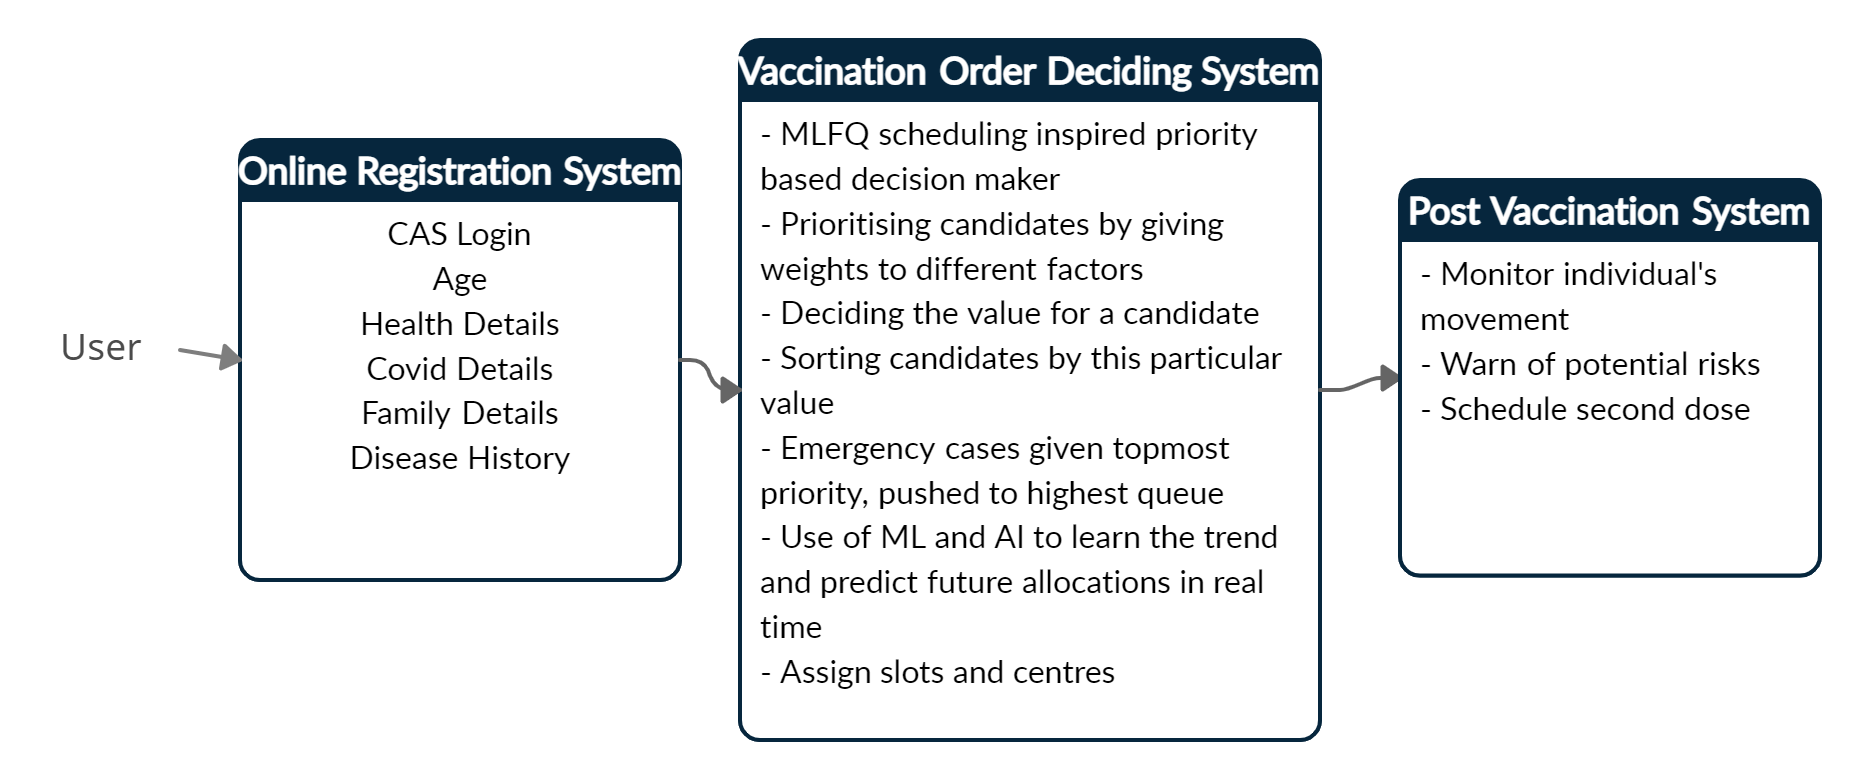
\includegraphics[width=9cm]{./images/Systems_Architecture.png}
	\caption{Architecture of Vaccination System}
	\label{fig:galaxy}
\end{figure}

\section{System Architecture}

As mentioned earlier, the entire vaccination system has 3 components:
\begin{enumerate}
	\item An online registration system
	\item  A rating system
	\item  A vaccination monitoring system
\end{enumerate}

\subsection{ Online Registration System}
A web portal with app support (Android/iOS) can be developed. Since we are currently focusing on vaccination within the college, we can use the Central Authentication System (CAS) which is already used extensively in our college. We also extend the support to Google or Facebook login for further support and authentication.

\subsubsection{Framework}
The registration portal can be make using technologies like MERN stack or Django, etc. College servers can be used to store data or server can be rented online, though use of college servers will provide better privacy. Similarly, for developing a smartphone app, technologies like Flutter can be used. The UI should a simple one, easy to use and clear with details required.

\subsubsection{Registration details}
Since we are mainly planning the system for college, we will use CAS details here. We already have details of every college member in our database. In case there is someone whose data is missing, a sign-up option will be available. The registration system will ask several details like covid status, covid symptoms, disease history, immunity prediction, family covid status, travel history, etc. Users will also be given choice of languages for details and to upload relevant documents. Technologies like NLP, AI and Image Reconnaissance can be used to extract useful data from the given information. This information is then stored in the college servers and fed into the decision-making system for determining the order of vaccination.

\subsection{Vaccination Order Deciding System}
Now we move on to the main essence required from the vaccination system, the order in which the candidates should be vaccinated. We take inspiration from the computer processors and schedulers which assign values to different processes based on priority and then decide which process to execute next. We look into some schedulers like PBS (Priority Based Scheduling), MLFQ(Multilevel Feedback Queue Scheduling), etc. Lets look into the functionality of these schedulers.
\begin{figure}[htp]
	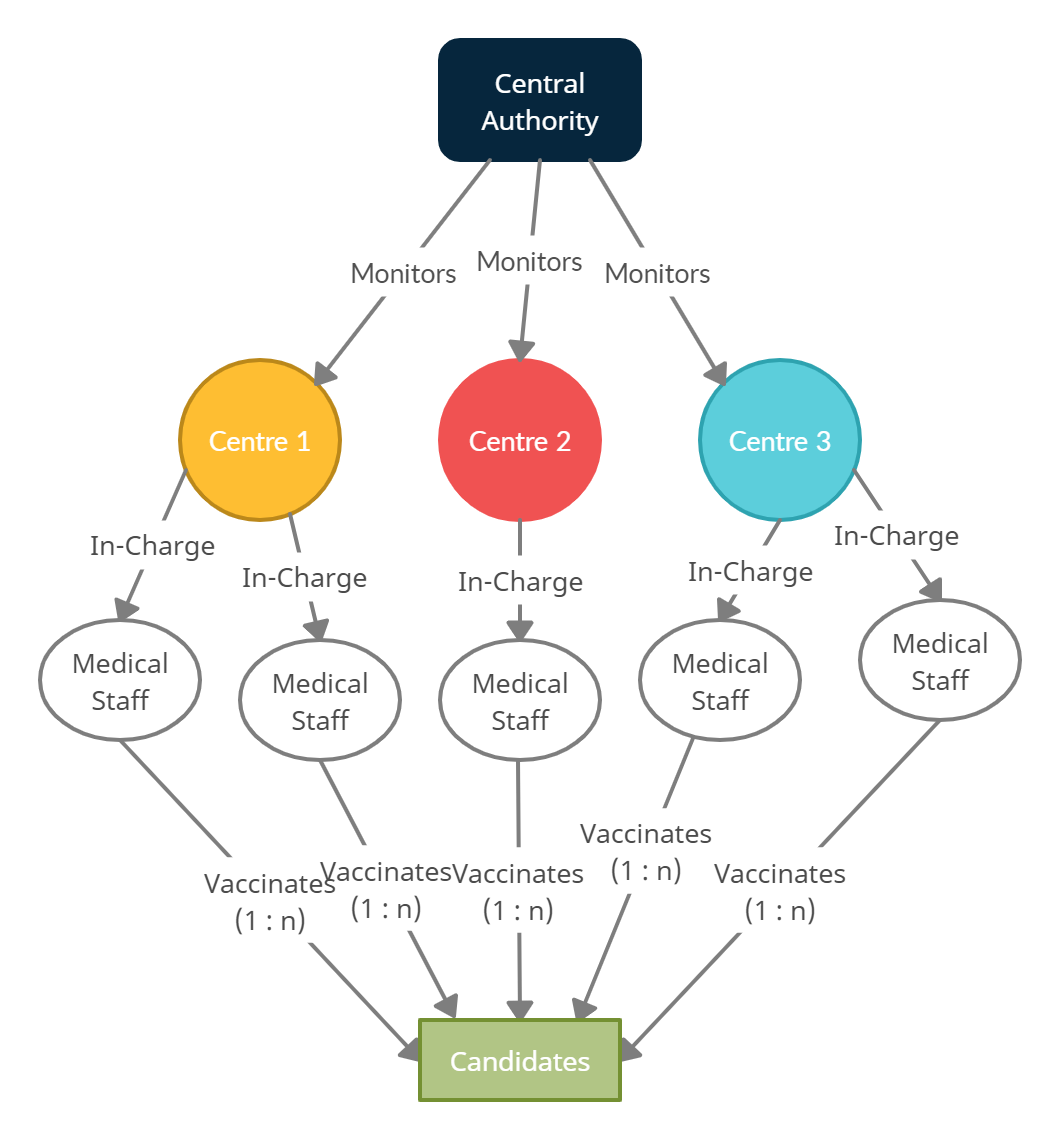
\includegraphics[width=9cm]{./images/Admin_structure.png}
	\caption{Administration Hierarchy}
	\label{fig:galaxy}
\end{figure}
\subsubsection{Priority Based Scheduling}
Priority Based Scheduling is a method of scheduling processes that is based on priority. In this algorithm, the scheduler selects the tasks to work as per the priority. The processes with higher priority should be carried out first, whereas jobs with equal priorities are carried out on a round-robin or FCFS basis. Priority depends upon memory requirements, time requirements, etc. In priority scheduling, a number is assigned to each process that indicates its priority level. In this type of scheduling algorithm, if a newer process arrives, that is having a higher priority than the currently running process, then the currently running process is preempted.

\subsubsubsection{Preemptive Scheduling vs Non-Preemptive Scheduling:}
In Preemptive Scheduling, the tasks are mostly assigned with their priorities. Sometimes it is important to run a task with a higher priority before another lower priority task, even if the lower priority task is still running. The lower priority task holds for some time and resumes when the higher priority task finishes its execution.

\subsubsection{Multilevel Feedback Queue Scheduling}\cite{MLFQ}

Unlike multilevel queue scheduling algorithm where processes are permanently assigned to a queue, multilevel feedback queue scheduling allows a process to move between queues. This movement is facilitated by the characteristic of the CPU burst of the process. If a process uses too much CPU time, it will be moved to a lower-priority queue. This scheme leaves I/O-bound and interactive processes in the higher priority queues. In addition, a process that waits too long in a lower-priority queue may be moved to a higher priority queue. This form of aging also helps to prevent starvation of certain lower priority processes

\subsubsubsection{Algorithm}
Multiple FIFO queues are used and the operation is as follows:
\begin{enumerate}
	\item A new process is inserted at the end (tail) of the top-level FIFO queue.
	\item At some stage the process reaches the head of the queue and is assigned the CPU.
	\item If the process is completed within the time quantum of the given queue, it leaves the system.
	\item If the process voluntarily relinquishes control of the CPU, it leaves the queuing network, and when the process becomes ready again it is inserted at the tail of the same queue which it relinquished earlier.
	\item If the process uses all the quantum time, it is pre-empted and inserted at the end of the next lower level queue. This next lower level queue will have a time quantum which is more than that of the previous higher level queue.
	\item This scheme will continue until the process completes or it reaches the base level queue.
\end{enumerate}
At the base level queue the processes circulate in round robin fashion until they complete and leave the system. Processes in the base level queue can also be scheduled on a first come first served basis. Optionally, if a process blocks for I/O, it is 'promoted' one level, and placed at the end of the next-higher queue. This allows I/O bound processes to be favored by the scheduler and allows processes to 'escape' the base level queue. When it comes to scheduling, the scheduler still begins at the top of the highest level queue. The scheduler can only take a process from the next lower level queue if the highest level queue is empty. Picking up in the subsequent lower level queues follows the same strategy. In the meantime, if a process enters one of the higher-level queues, it will take precedence over a process in the lower-level queue.

\subsubsubsection{Scheduling parameters}
In general, a multilevel feedback queue scheduler is defined by the following parameters:
\begin{enumerate}
	\item The number of queues.
	\item The scheduling algorithm for each queue which can be different from FIFO (First In First Out).
	\item The method used to determine when to promote a process to a higher priority queue.
	\item The method used to determine when to demote a process to a lower priority queue.
	\item The method used to determine which queue a process will enter when that process needs service.
\end{enumerate}
Upon closer inspection, we see that MLFQ would be an ideal scheduler for our vaccination system.

\subsubsection{Prioritising the candidates}
Now looking upon the various factors related to a candidate, first and foremost, we prioritise the candidates on the basis of their covid status. This means that people with serious conditions who are in urgent need of vaccination will receive the highest priority, surpassing everyone else. Next, certain weight factors will be assigned to other parameters like time of registration, age, probability of effectiveness due to past medical history, how close a person has been with a covid positive person, whether someone from the family of a person has been covid positive or not (since this increases the person’s chance of being affected by covid). We add up the different weights and come up with a value. This value is then sorted and individuals with higher values are given higher priority. Of course, as seen in MLF! Scheduling, as time passes, a weight of time also keeps on adding and priorities from one level are shifted to another level. Also in case an emergency comes up during vaccination of normal individuals, it is given the max priority and rest individuals are pushed to the next lower priority queue.

\subsubsection{Theory behind Calculation of Priority Values}
To calculate the score, consider $w_{1}$ as weightage of Age factor $A$, $w_{2}$ as weightage of probability of covid symptons $S$, $w_{3}$ as weightage of probability of contact with covid positive person $C$, $w_{4}$ as weightage of negative side effects of vaccine $N$ ($N$ being a negative value here), other factors as $X$ and in case of machine learning, some contribution of past data $D$ as $w_{5}$.
\\Let $PV$ be Priority Value obtained. Then,
\begin{equation}
	PV = {w_{1}*A + w_{2}*S + w_{3}*C + w_{4}*N + X + w_{5}*D} 
\end{equation}
Of course, we are considering a simple linear relation here but the relation can be of higher degree too. Higher the Priority Value, higher will be the precedence of the candidate.
\subsubsection{Use of Machine Learning}
Machine learning can play a vital part here, since it can learn from the pattern of assigning different weights to different factors and apply it for predicting the future cases. Thus, once we accumulate enough data and the validation reaches a satisfactory level, the portal could be trained to identify the priority of an individual as soon as he/she enters the details and can provide them a slot then and there, instead of taking time to evaluate later. With help of machine learning, the system can also account for new factors and change the weights of different factors accordingly, without any intervention of humans. For instance at certain point of time, age might be given more weightage but as conditions change, the factor of ‘proximity to a covid positive person’ or ‘covid symptoms’ might be given more weightage while age could be given less weightage. Thus, all these conditions will help training the AI and look for best possible route for the future.
\begin{figure}[htp]
	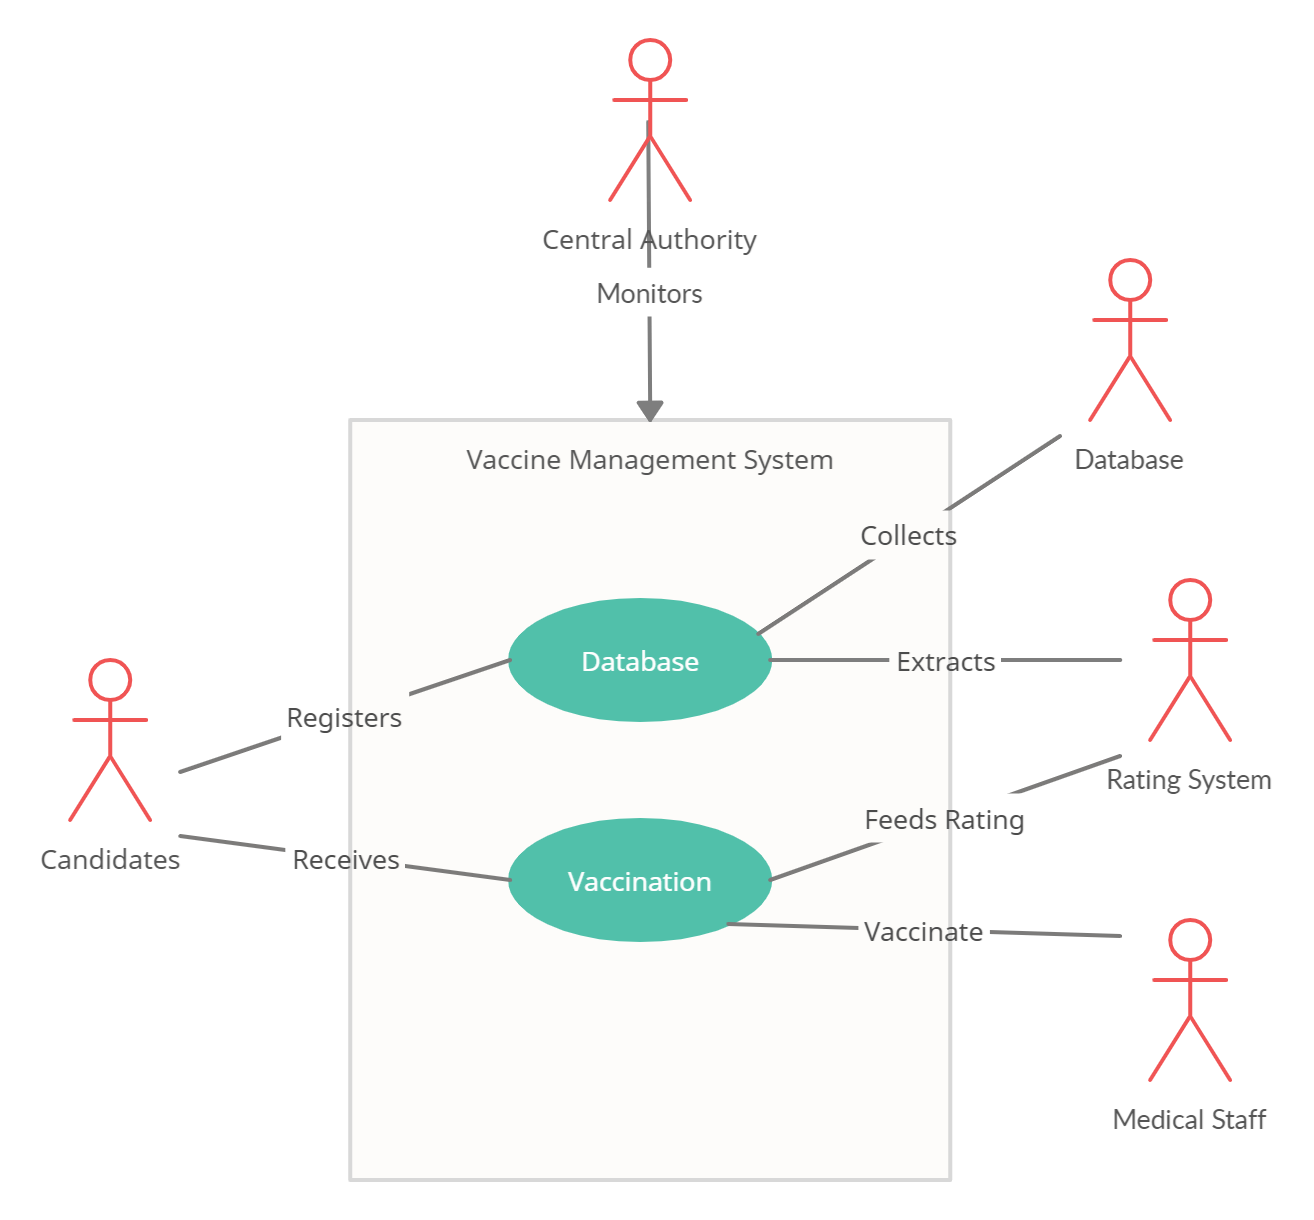
\includegraphics[width=9cm]{./images/use_case_diagram.png}
	\caption{Use Case Diagram}
	\label{fig:galaxy}
\end{figure}
\subsubsection{Assigning of Slots and Vaccination centres}
There can be many centres setup across the campus and can have multiple factors of differentiation. Some centres could be for high risk individuals, some can be for emergency patients while some can be common for all candidates. The crowd pressure and the supply of vaccines to these centres will be regularly monitored by a central committee, such that neither there is shortage of vaccine at any centre nor there is excess, unusable vaccines at any centre. Also, it has to be taken care that the number of people at a particular centre at a particular time has to be maintained at a safe level.

\subsection{Post Vaccination Management System}

Vaccination of individuals was half the battle; the risk of covid outbreak will still be present. Thus it is equally important to monitor individuals so that they remain in their own safe bubble. We can use technologies like GPS and Bluetooth to monitor the position of individuals and alert them in case they come in dangerous proximity to a probable covid affected person. This system will also track the post-vaccination health of individuals and monitor the effects of vaccines. This all can be done using the portal where users can be allowed to provide details of post-vaccination effects on their body. Again, this data could be used to train AI so that it can predict vaccination for individuals with similar health issues. Also, this system can be used to decide the second dosage of vaccines for the candidates, again working on several factors, this time including an important factor of time duration from first dose as the vaccines are most effective if given within a certain time period.

\section{Conclusion}
This solution provides an effective and efficient Vaccination and Management System for the Institute. It takes care of every aspect and every flaw present in the current vaccination system run by the government. With the help of modern technology and Artificial Intelligence, I have no doubt that we can definitely be successful in our vaccination program. 

\begin{thebibliography}{9}

\bibitem{highcourt} 
\href{https://www.ndtv.com/india-news/delhi-high-court-says-wastage-of-covid-19-vaccine-in-current-situation-criminal-2418287}{Wastage Of COVID-19 Vaccine In Current Situation ''Criminal'': Delhi High Court}

\bibitem{vigilanz}
\href{https://vigilanzcorp.com/}{Vigilanz Corporation}

\bibitem{temp1}
\href{https://swachhindia.ndtv.com/indias-covid-19-vaccination-programme-explained-what-is-co-win-vaccine-delivery-management-system-all-you-need-to-know-55043/}{India’s COVID-19 Vaccination Programme Explained}

\bibitem{uchealth}
\href{https://biointellisense.com/biobutton}{BioIntelliSense BioButton Vaccine Monitoring Solution}

\bibitem{docasap}
\href{https://docasap.com/}{DocASAP}

\bibitem{MLFQ}
\href{https://www.geeksforgeeks.org/multilevel-feedback-queue-scheduling-mlfq-cpu-scheduling/}{Multilevel Feedback Queue Scheduling }

\bibitem{}
\href{https://www.tutorialspoint.com/operating_system/os_process_scheduling_algorithms.htm}{Operating System Scheduling algorithms
}

\bibitem{usc}
\href {https://news.usc.edu/181226/artificial-intelligence-ai-coronavirus-vaccines-mutations-usc-research/}{Artificial intelligence aims to outsmart the mutating coronavirus}

\end{thebibliography}

\end{document}